\chapter{Modeling}

\section{Problem domain}
For this analysis we will follow the Object Oriented Analysis of the problem domain approach. We have made an event table to better understand what we need in our program and from that we have made a class diagram and state diagram. This give an overview of what we would have to implement in our program and the class diagram describe, how the base model would look like. 

\subsection{Event table}
To do the event table, see figur \vref{fig:event_table}, we came up with potential classes in the problem domain and events that would happen in the application domain. First all the potential classes was written down and then we evaluated each class with meant that some classes was abandoned. One of classes that were abandoned the Autistic Child because in the model it is the child's mobile device that identifies the child and thereby the class Autistic Child was redundant. Classes such as Application and specific applications were used in the table because of the \textbf{system definition} %(check at det passer senere)
system definition to e.g. be able edit the settings or make events in the calendar. Archives and specific archives were added because the use of PECS is essential for at least two applications and they will be stored in categories such that the parents quickly would be able to find the wanted PECS. On the mobile device a database would be installed from which the program's for the child is installed and therefore the database is also important.

\begin{figure}[h]
	\centering
		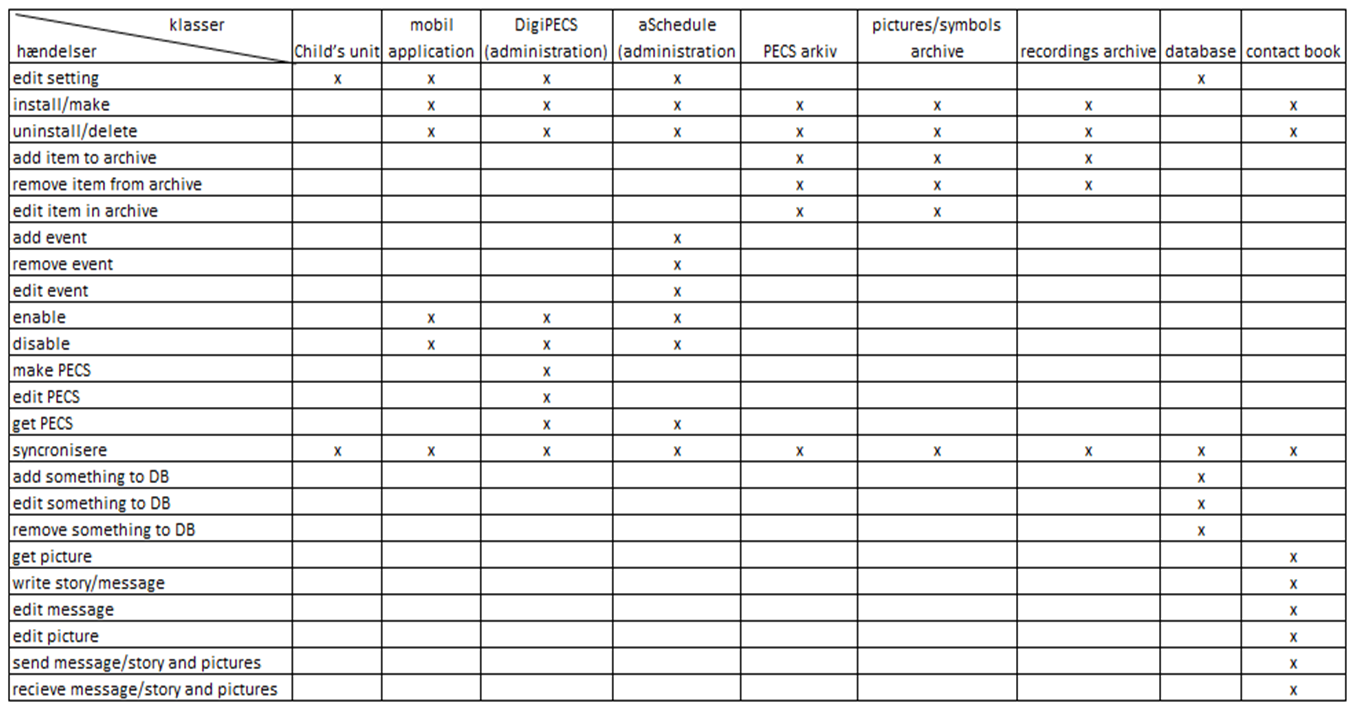
\includegraphics[width=1.0\textwidth]{img/event_table.png}
	\caption{event table }
	\label{fig:event_table}
\end{figure}

Many potential events were also considered and then evaluated which also meant that not all events was used in the table. The event take a picture was considered, but the action of taking this picture seemed not relevant until it was add to one of the archive despite its origin and therefore it was left out. However, the event that was used also could be used multiple times such as add/edit/delete a picture/recoding/text or all of the application would at a time be installed and uninstalled. All of the applications should also be able to become disabled and enabled again for the child within a time periods according to \textbf{�the others project� }. %find et reference punkt
The application aSchedule should be able to add new events into the calendar and this event can be edited or delete and it should be able to use the PECS from the archive. The application DigiPECS should make the PECS by connecting a picture, a sound/recording and some text and the user should also be able to edit and delete it. The application should also be able to save a complete PECS in the archive which is a distinction from making one. 

The administrator program would also have to be able to synchronize everything on the mobile device to match the changes made on the computer that can be done for the application, archives and database.  The contact book should be able to send and receive message/stories about the child's day and include pictures.  

   
\subsection{Class diagram}
After the event table completion we made a class diagram that shows how the classes are connected, see figur \vref{fig:class_diagram}. We have the child's unit at the top of the hierarchy which in our model is a composition of applications, archives and a database. From the applications class we know that we need some subclasses that specify what the program can. These subclasses could be e.g. DigiPECS, aSchedule and contact book. The archives could also be specified into subclasses for archive contain picture, recording or PECS. Obviously contain the Picture archive pictures, and Recordings archive contains recordings and sounds while the PECS archive contain PECS units. However, note that a PECS is a composition of one picture, one recording and some text which is the reason for the association between PECS and Picture, as well as PECS and Recording.


There is also an association between the applications and the archives because the programs should be able to use the contents of the archives. E.g. DigiPECS should be able to use and edit pictures, recordings and PECS units while aSchedule only should be able to use PECS units. The database contains the application which the child can use and therefore is a composition for non or more applications.
\begin{figure}[h]
	\centering
		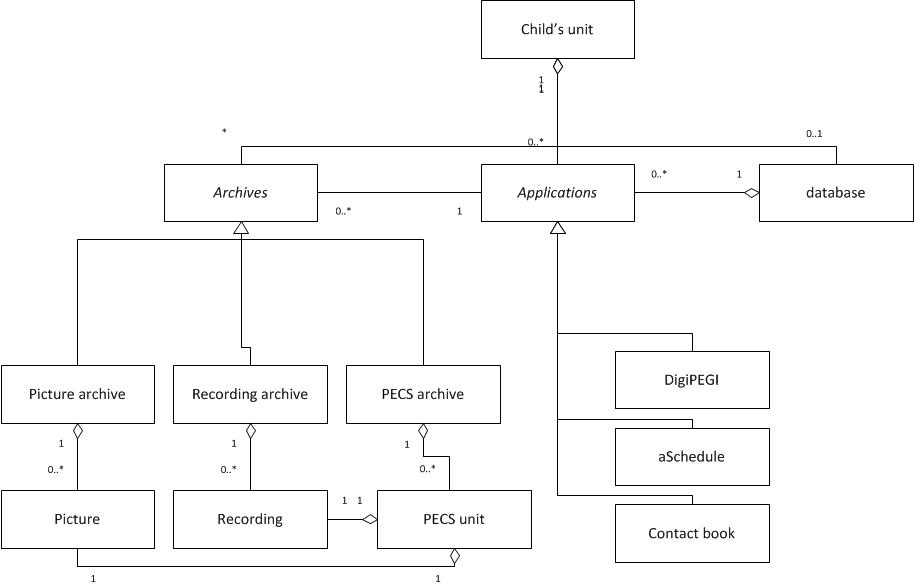
\includegraphics[width=1.00\textwidth]{img/class_diagram.jpg}
	\caption{class diagram}
	\label{fig:class_diagram}
\end{figure}


\subsection{State diagram}
In a state diagram it is shown how a class behaves, we have made a state diagram for the most important classes. For all the applications its general behavior is that it can edit the setting, enable and disable the applications on the mobile device in a time period. 

\subsubsection{Contact book}
\begin{figure}[h]
	\centering
		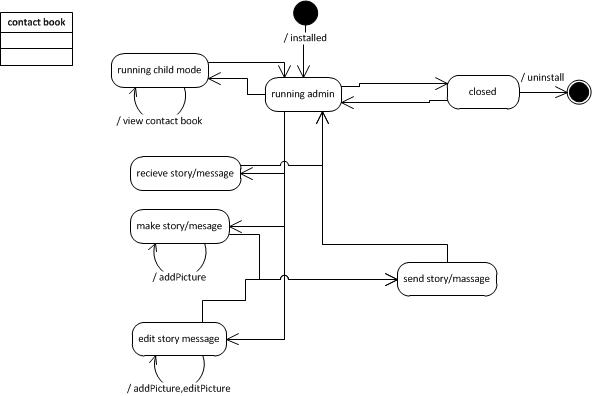
\includegraphics[width=0.75\textwidth]{img/contact_book.jpg}
	\caption{state diagram of the contact book}
	\label{fig:contact_book}
\end{figure}

First the class Contact book's behavior(see \vref{fig:contact_book}) starts with its installation and it is able to run in two modes the child running mode where the guardians' and the child can see the pictures and the story to talk about it.  The other mode is only for the guardian and kindergarten teacher who would be able to send and receive messages or stories with pictures about the child e.g. about the child's day or a message saying that the child is ill today. The guardian or kindergarten teacher would have to make a new message or edit another and add pictures to it, before sending it. The behavior ends when the user uninstall it (skal revideres).  

\subsubsection{aSchedule}
\begin{figure}[h]
	\centering
		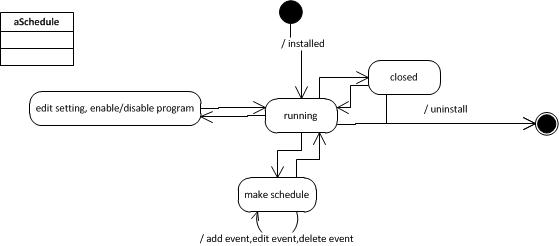
\includegraphics[width=0.75\textwidth]{img/aSchedule.jpg}
	\caption{state diagram of the aSchedule}
	\label{fig:aSchedule}
\end{figure}

Another class is the aSchedule(see \vref{fig:aSchedule}) after the installation its behavior is primarily to make, edit and delete events in the calendar and it also have the general behavior. 

\subsubsection{DigiPECS}
\begin{figure}[h]
	\centering
		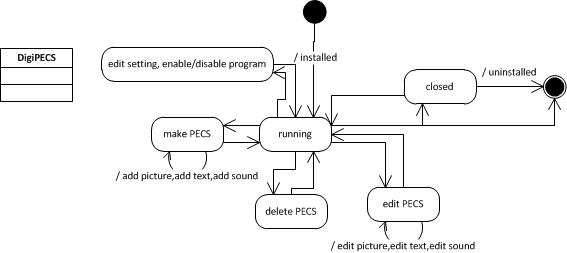
\includegraphics[width=0.75\textwidth]{img/digiPECS.jpg}
	\caption{state diagram of the DigiPECS}
	\label{fig:digiPECS}
\end{figure}
The last state diagram is made for the DigiPECS(see \vref{fig:digiPECS}) which is able to make, edit and delete the PECSs in the archive which then can be used by the child and user to communicate with.      
 
